\chapter{Resultados Obtidos}
\label{chap:resultadosObtidos}

Neste capítulo, é apresentado as primeiras aplicações do catálogo, para isso então foi utilizado o conceito de personas \ref{sec:personas} buscando demonstrar os cenários em que o catálogo pode ser aplicável. Portanto, realizou-se a simulação de cinco cenários para validar a aplicação do Catálogo de Segurança. 

O capítulo é divido inicialmente pelos cenários contextualizados dentro de cada persona. Os cenários tem, a descrição da persona, identificação da possível solução (Quando necessário descrever para o cenário) e aplicação do catálogo, finalizando o capítulo é apresentado a primeira visão da aplicação do catálogo.  


\section{Cenário 1}
\label{subsec:persona1}

Heleno, 24 anos, Engenheiro de Requisitos está assumindo a função de elicitar os requisitos não funcionais para um novo projeto na empresa em que trabalha, o projeto será desenvolvido em \textit{Rails} e seu chefe pediu que devesse ter perfis diferentes dentro da aplicação sendo os perfis de membro e administrador. O sistema ao qual seu chefe está solicitando deve principalmente ser um sistema seguro para autenticação do usuário com capacidade de redefinir a senha do usuário, ser possível monitorar a quantidade de entradas do usuário e por final validar email do usuário.

\begin{itemize}
	\item O problema: Mapear os métodos de autenticação relevantes na autenticação do usuário. 
	\item Objetivo: Verificar o nível de satisfação de segurança da autenticação. 
	\item Desafio: Análise dos impactos entre os requisitos não funcionais para autenticar os usuários.
\end{itemize}


\subsubsection{Identificar possível solução}

O problema principal do usuário é a realização da autenticação do usuário o primeiro passo a ser adotado é identificar qual \textit{gem} é a mais adequada, segundo o \textit{The Ruby Toolbox} na categoria \textit{Rails Authentication} o ranking de popularidade das três \textit{gems} mais utilizadas para autenticação é \cite{rubytoolbox}:

\begin{enumerate}
	\item devise: 38.982.741 downloads
	\item omniauth: 23.524.509 downloads
	\item doorkeeper: 7.091.328 downloads
\end{enumerate}

Portanto, a \textit{gem} selecionada para ser aplicada ao projeto por Heleno é a \textit{devise}, pois além da posição do ranking é a \textit{gem} mais recomendada pela comunidade. As vantagens da utilização do \textit{devise} é  (i) uma solução baseada no padrão arquitetural MVC, (ii) permite a criação e a utilização de vários perfis de usuários conectados ao mesmo tempo, (iii) basea-se no conceito de modularidade, utilizando somente o que é necessário. Essa \textit{gem} possui 10 módulos \cite{gemdevise}: 

\begin{enumerate}
	\item \textit{Database Authenticatable}: \textit{Hashes} que armazenam a senha no banco de dados para serem validadas durante o \textit{login}. A autenticação pode ser realizada via método POST ou HTTP \textit{basic authentication}. 
	\item \textit{Omniauthable}: Suporte adicional ao \textit{omniauth}.
	\item \textit{Confirmable}: Envio automático de email para confirmação da conta e verificação da confirmação da conta durante o \textit{login}.
	\item \textit{Recoverable}: Envia instruções de redefinição de senha para o usuário e redefine a senha do usuário.
	\item \textit{Registerable}: Permite a inscrição de usuários por meio do processo de registros, permitindo a edição e a remoção de suas contas.
	\item \textit{Rememberable}: Gerenciador de \textit{token} para notificar o usuário da existência de \textit{cookie} salvo.
	\item \textit{Trackable}: contador de entradas, mantendo o registro de data, hora e endereço de IP.
	\item \textit{Timeoutable}: Expira as sessões inativas em um período de tempo especificado. 
	\item \textit{Validatable}: Validações de email e senha. 
	\item \textit{Lockable}: Bloqueia a conta após exceder o número de tentativas especificado, portanto o desbloqueio pode ocorrer via email ou após um período de tempo. 
\end{enumerate}

\subsubsection{Aplicação do Catálogo de Segurança}

Através dos módulos apresentados anteriormente é possível realizar o mapeamento deles utilizando o catálogo, então, modelou-se a \textit{gem devise} e seus respectivos métodos como operacionalizações no catálogo. 

\pagebreak

\begin{figure}[h!]
	\centering
	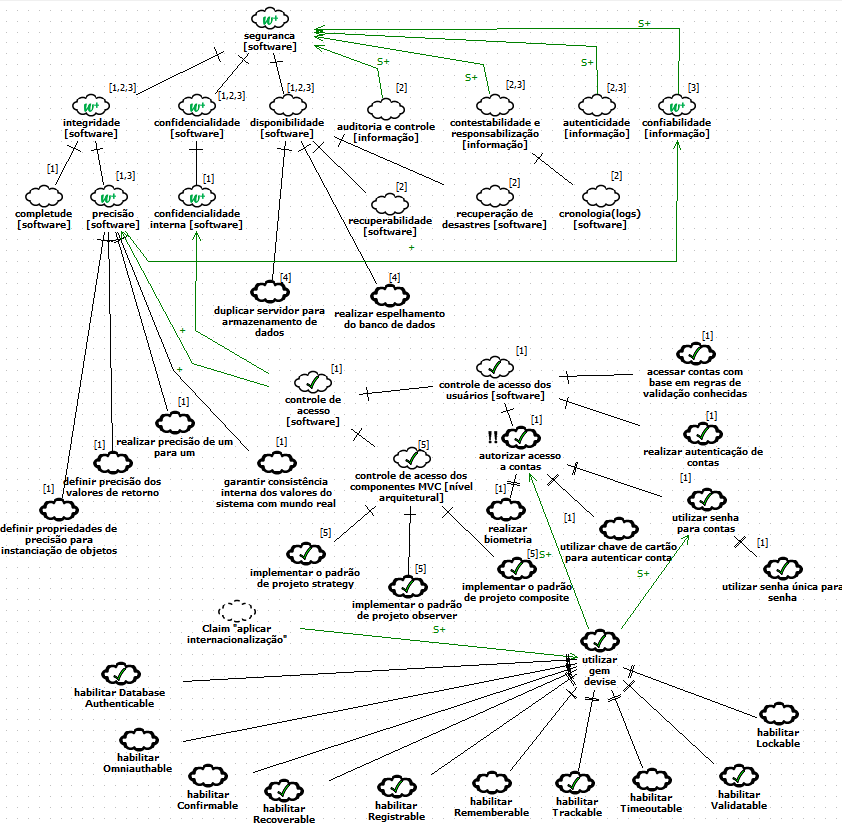
\includegraphics[keepaspectratio=true,scale=0.7]{figuras/catalogoPersona1.PNG}
	\caption{Operacionalizações para autenticação de usuário utilizando a \textit{gem devise}.}
	\label{catalogoPersona1}
\end{figure}


O Catálogo de Segurança aplicado no cenário 1 é apresentado na \ref{catalogoPersona1}, onde as operacionalizações são incrementadas no Catálogo de Segurança respeitando os módulos da \textit{gem devise}, a operacionalização  “autorizar acesso a contas” passou a possuir grau de prioridade alto, porquê é uma das operacionalizações que impactam diretamente a solução para o problema. 

É então possível utilizando a notação do NFR \textit{Framework} realizar a modelagem da \textit{gem devise} como uma operacionalização, representando a existência de alguma contribuição positiva (SOME+) com as operacionalizações  “autorizar acesso a contar” e “utilizar senha para contas”.
 
As operacionalizações filhas de “utilizar \textit{gem devise}” e que atendem as necessidades da persona descrita no cenário 1 são:

\begin{itemize}
	\item “habilitar \textit{Database Authenticable}”: É um dos requisitos mínimos para que ocorra a persistência da senha no banco de dados.
	\item “habilitar \textit{Recoverable}”: Capacidade de redefinir a senha do usuário.
	\item “habilitar \textit{Registrable}”: É um dos requisitos mínimos e que permite a inscrição de usuários. 
	\item “habilitar \textit{Trackable}”: monitorar a quantidade de entradas do usuário. 
	\item “habilitar \textit{Validatable}”: Validar conta via email do usuário. 
\end{itemize}

Portanto ao habilitar os módulos da \textit{gem devise} dentro da camada \textit{model} nas classes \textit{Admins} e \textit{Members}, as operacionalizações são satisfeitas. Podemos então verificar qual nível de satisfação da segurança do software pode alcançado com a utilização da \textit{gem devise}. O trecho de código abaixo apresenta como habilita-se os módulos.  
 

\begin{lstlisting} 
class Admins < ApplicationRecord
devise :database_authenticatable, :registerable,
:recoverable, :rememberable, :trackable, :validatable
end 
\end{lstlisting} 

A implementação dos padrões de projeto \textit{strategy}, \textit{observer} e \textit{composite} já estão satisfeitos pois a aplicação é desenvolvida com o framework rails que obedece o padrão MVC e a \textit{gem} que está sendo utilizada também percorre todas as camadas. 

\section{Cenário 2}
\label{subsec:persona2}

Pedro, 23 anos, Engenheiro de Software, trabalha em empresa privada e possui a necessidade de desenvolver o sistema da ouvidoria da instituição, tal sistema deverá ser desenvolvido em plataforma web para atender os processos de manifestação (denúncia, reclamação, solicitação, sugestão e elogio) realizados pela ouvidoria. Esse tipo de informação deve ser estritamente confidencial, podendo ou não o manifestante ser anonimo.  

\subsection{Identificar possível solução}

Uma possível solução é gerar um número de protocolo durante o registro da manifestação para que possa ser realizado o acompanhamento, o número de protocolo será utilizado tanto para a manifestação anônima quando para a manifestação formal. O manifestante poderá acompanhar o status de sua manifestação através da visão de acompanhamento de manifestação, onde ficará registrado as respostas dadas pela ouvidora.

A Ouvidora no caso acessará o sistema de forma diferente, utilizando a área administrativa do sistema através de autenticação de usuário, onde permite que a mesma visualize todas as manifestações permitindo então a seleção da manifestação desejada para que seja possível a redação da resposta para o manifestante.  


\subsection{Aplicação do Catálogo de Segurança}

\begin{figure}[h!]
	\centering
	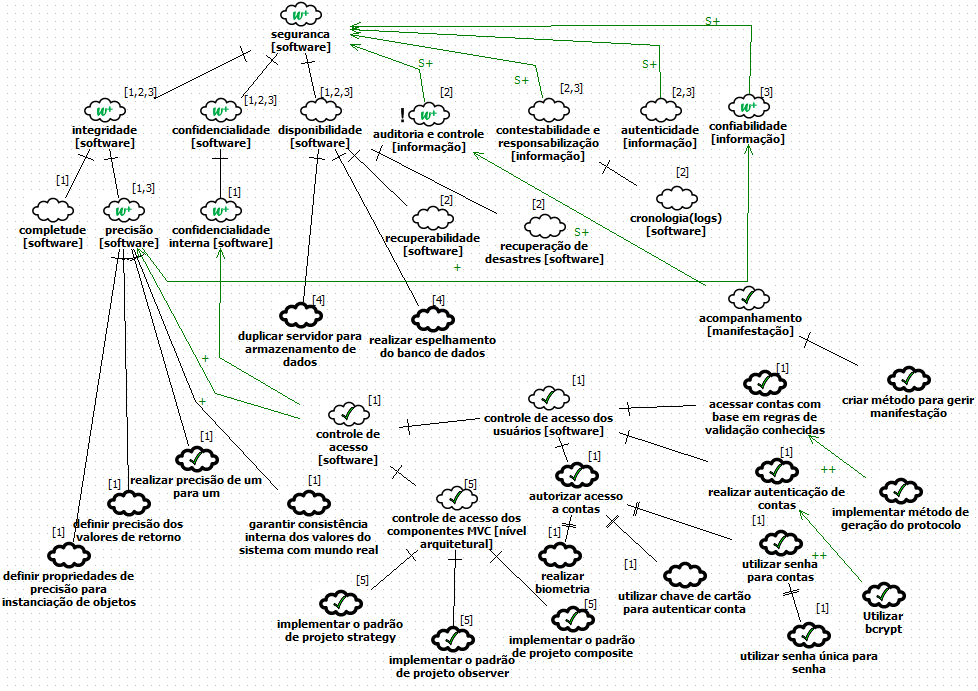
\includegraphics[keepaspectratio=true,scale=0.65]{figuras/catalogoPersona2.PNG}
	\caption{Catálogo de segurança aplicado ao sistema de ouvidoria.}
	\label{catalogoPersona2}
\end{figure}



Na aplicação do Catálogo de Segurança da figura \ref{catalogoPersona2} teve-se a necessidade de focar em  “auditoria e controle”, pois o cenário demandava  o acompanhamento das manifestações pelos ouvidores, portanto foi expandido no catálogo uma nova meta flexível “Realizar acompanhamento das manifestações” e uma operacionalização “Criar método para gerir manifestação”, a operacionalização é definida pelos métodos implementados na \textit{controller - ManagerManifestationsController}. Portanto a meta flexível “auditoria e controle” é suficientemente satisfeita para este contexto.

Para que a meta flexível “controle de acesso dos usuários” seja suficientemente satisfeita temos três operacionalizações que são suficientemente satisfeitas e que estão no nível mais baixo no Catálogo de Segurança, são elas: (i) “Implementar método de geração do protocolo”: Trata-se do método para gerar os números de protocolos com caracteres (de “a” à “z”), (de “A” à “Z”) e (de “0” à “9”) utilizado para compor um número de protocolo de 10 digitos; (ii) “utilizar senha única para senha”: Para cada usuário administrador/ouvidor cadastrado no sistema é gerada uma única senha para autenticação; e (iii) “utilizar bcrypt”: Trata-se de uma \textit{gem} que utiliza algoritmo de \textit{hashing} criptográfico que trata um trecho do dado para gerar um \textit{hash}, pois ao gerar uma senha dessa maneira trata-se da execução de um processo não reversível porquê não há como voltar da \textit{hash} para a senha \cite{brcypt}.

A operacionalização “realizar precisão de um para um” é suficientemente satisfeita pois para cada manifestação ocasionada por determinado evento de manifestação do mundo real existirá uma única manifestação no sistema.

Observa-se portanto que a segurança do software é parcialmente satisfeita devido a satisfação parcial da integridade do software e da confidencialidade, ocorridos devido aos níveis de satisfação das metas flexíveis e operacionalizações em níveis mais baixos do Catálogo de Segurança. 

\section{Cenário 3}
\label{subsec:persona3}



Milena, 22 anos, Engenheira de Software, possui várias atividades no seu dia-a-dia, sentiu-se então a necessidade de organizar as atividades e para isso devido suas habilidades decidiu escrever um programa para obter maior controle. Esse programa permite a inserção com descrição da atividade, a data de início, a previsão de conclusão e o status da atividade. Portanto, Milena optou por fazer seu sistema em rails e decidiu verificar as relações entre as camadas do sistema com o foco em segurança.

\begin{itemize}
	\item O problema: Atividades diárias desorganizadas;
	\item Objetivo: Desenvolvimento de sistema para auxiliar na organização das atividades;
	\item Desafio: Verificar as relações entre as camadas do sistema com foco em segurança.
\end{itemize}

\subsubsection{Aplicação do Catálogo de Segurança}

Na descrição da persona tem se a necessidade de vincular cada atividade do mundo real com uma entidade no sistema, para isso utilizou-se o comando \textit{scaffold} do rails, tal comando gera a estrutura de arquivos de acordo com o padrão MVC, gerando o \textit{model}, o \textit{controller}, as \textit{views} necessárias \cite{railscommunity}. 

\begin{figure}[h!]
	\centering
	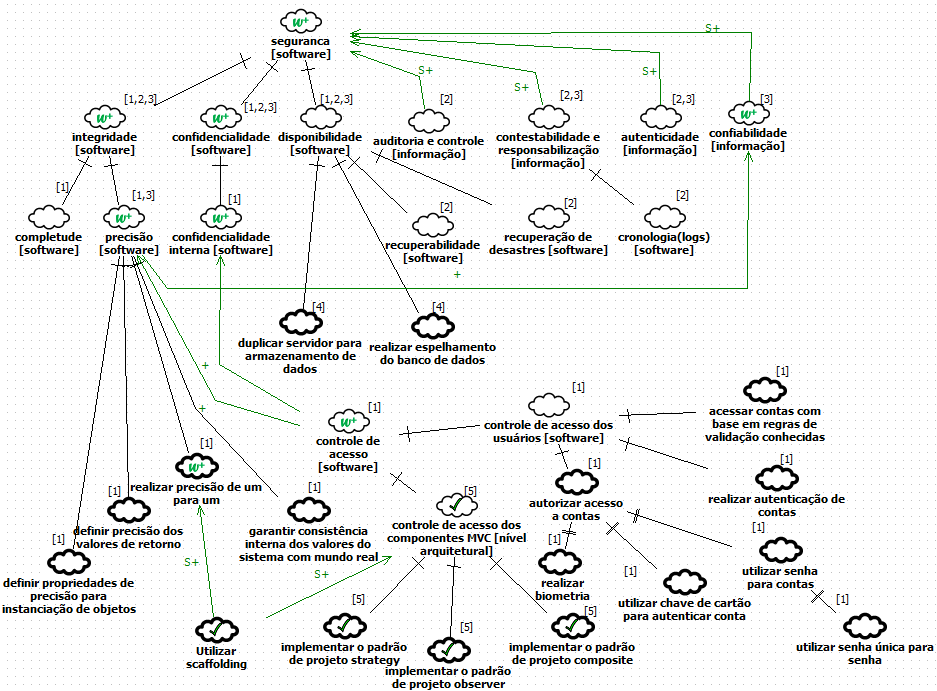
\includegraphics[keepaspectratio=true,scale=0.7]{figuras/catalogoPersona3.PNG}
	\caption{O scaffolding do rails no Catálogo de Segurança.}
	\label{catalogoPersona3}
\end{figure}


\section{Cenário 4}
\label{subsec:persona4}


Gustavo, 23 anos, Engenheiro de Requisitos de empresa privada, possui a demanda de analisar os requisitos do sistema de solicitação de documentos digitais via plataforma web, tal sistema possui arquitetura MVC e está em constante evolução. 

Portanto seu chefe solicitou que o mesmo fizesse uma analise dos requisitos com foco na segurança do sistema, devido a emissão de documentos com assinatura digital. 

\subsection{Identificar possível solução}

A aplicação do Catálogo de Segurança pode ser uma das maneiras em que pode demonstrar a relação entre os RNF do sistema, principalmente quando o RNF que está em foco é segurança.

\pagebreak

\subsection{Aplicação do Catálogo de Segurança}

\begin{figure}[h!]
	\centering
	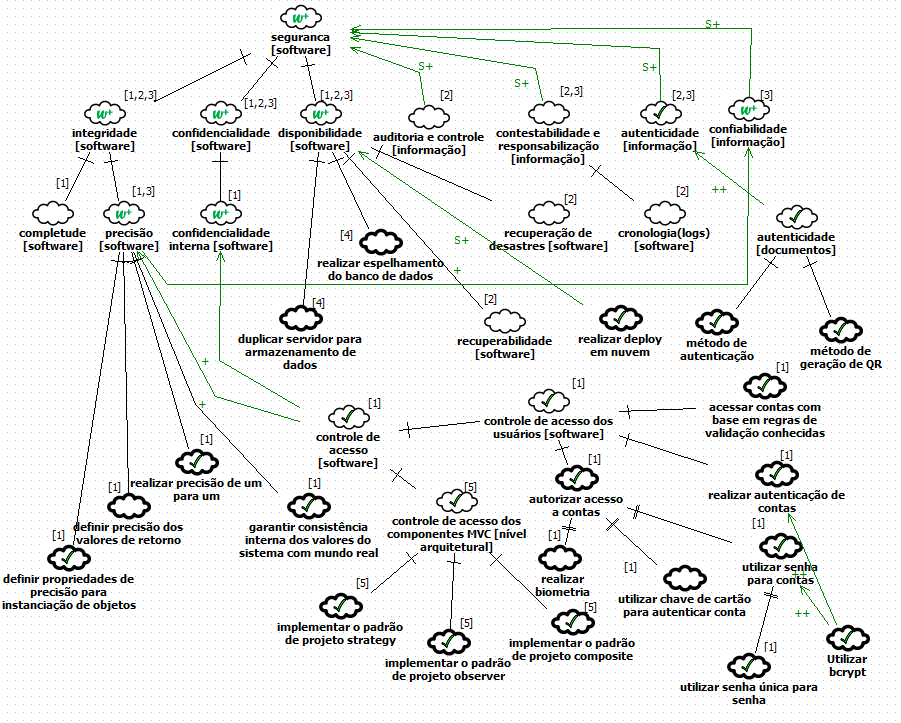
\includegraphics[keepaspectratio=true,scale=0.7]{figuras/catalogoPersona4.PNG}
	\caption{Catálogo aplicado a sistema de geração de documentos digitais.}
	\label{catalogoPersona4}
\end{figure}

A aplicação do catálogo apresentado na figura \ref{catalogoPersona4} possui uma extensão devido a utilização de assinatura digital nos documentos, que é modelada como uma meta flexível que está suficientemente satisfeita, pois depende de duas operacionalizações. As operacionalizações fazem uma relação do tipo AND com a meta flexível e ambas estão suficientemente satisfeitas sendo elas “método de geração de (\textit{Quick Response} Quick) QR” e o  “método de autenticação” que utiliza valores como o identificador do usuário e a \textit{string} do QR. Essas relações satisfazem suficientemente meta flexível para autenticidade da informação. 

O controle de acesso do software é satisfeito devido a relação das metas flexíveis e operacionalizações da mesma forma que os cenários \ref{subsec:persona2} e \ref{subsec:persona1} anteriores que já apresentaram os mesmos relacionamentos, com mesmos níveis de satisfação.  

Já a operacionalização “definir propriedades de precisão para instanciação de objetos”, é escrita em cada \textit{model} onde o \textit{rails} permite escrever os parâmetros para controle de instanciação dos objetos, neste cenário foi aplicado que o atributo da classe tem que existir no banco de dados, não podendo colocar vazio ou nulo. 

A aplicação está em um servidor do google na nuvem, garantindo sua disponibilidade, satisfazendo então suficientemente a operacionalização “realizar deploy em nuvem”. 

Semelhante as aplicações dos cenários \ref{subsec:persona2} e \ref{subsec:persona3} a “precisão de um para um” é suficientemente satisfeita. 

\section{Cenário 5}
\label{subsec:persona5}

Chung, 40 anos, Engenheiro de Software possui em seu quadro de responsabilidades a função de realizar manutenção e evolução de um dos sistemas ao qual é responsável. Portanto percebeu que um de seus sistemas poderia ficar indisponível caso ocorre-se algum problema no servidor de banco de dados, preocupado então com a segurança de seus sistemas, utilizou se o catálogo para analisar o impacto que o espelhamento da base de dados poderia afetar na segurança do software como um todo. 

\subsection{Aplicação do Catálogo de Segurança}

\begin{figure}[h!]
	\centering
	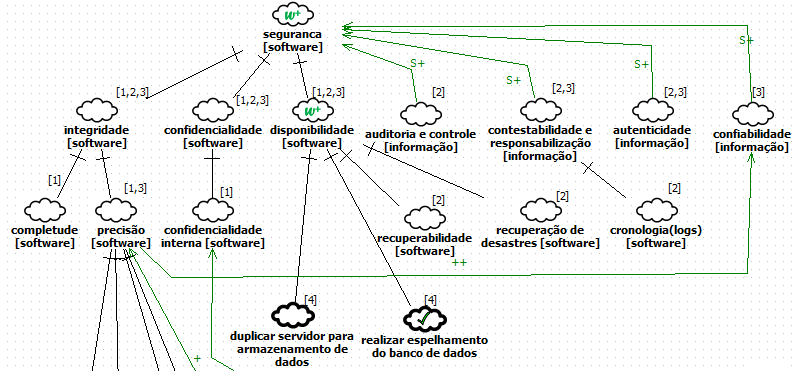
\includegraphics[keepaspectratio=true,scale=0.7]{figuras/catalogoPersona5.PNG}
	\caption{Catálogo de Segurança aplicado ao contexto de duplicação de base de dados.}
	\label{catalogoPersona5}
\end{figure}

Logo a operacionalização “espelhamento da base de dados” é suficientemente satisfeita, satisfazendo parcialmente a disponibilidade do software. Este cenário em especial foi modelado justamente para demonstrar o impacto de ações realizadas na base de dados na segurança do software.


\section{Primeira visão do Catálogo de Segurança após as aplicações nos cenários}
\label{sec: aplicacaoDoCatalogo}

Ao modelar o catálogo de segurança pela primeira vez sem ter realizado nenhuma interação com algum tipo de cenário obteve-se visão preliminar sobre Segurança devido a subjetividade e o conjunto de conceitos abstratos presentes na literatura. Isso é demonstrado no Capítulo \ref{chap:proposta} que detalha a construção do catálogo, permitindo chegar somente no primeiro e segundo nível de detalhamento. 

Ao aplicar os cenários para demonstrar a aplicação do catálogo observou-se que o Catálogo de Segurança permite não somente a visão preliminar da segurança de software, mas também de segurança da informação.

Como o Catálogo de Segurança foi aplicado em cenários onde a ferramenta de suporte ao desenvolvimento era o \textit{rails}, pode-se abstrair o Catálogo de Segurança para aplicações em \textit{rails}, demonstrando então a adaptabilidade do catálogo, como pode ser visualizado na Figura \ref{catalogoFull}.

\begin{figure}[h!]
	\centering
	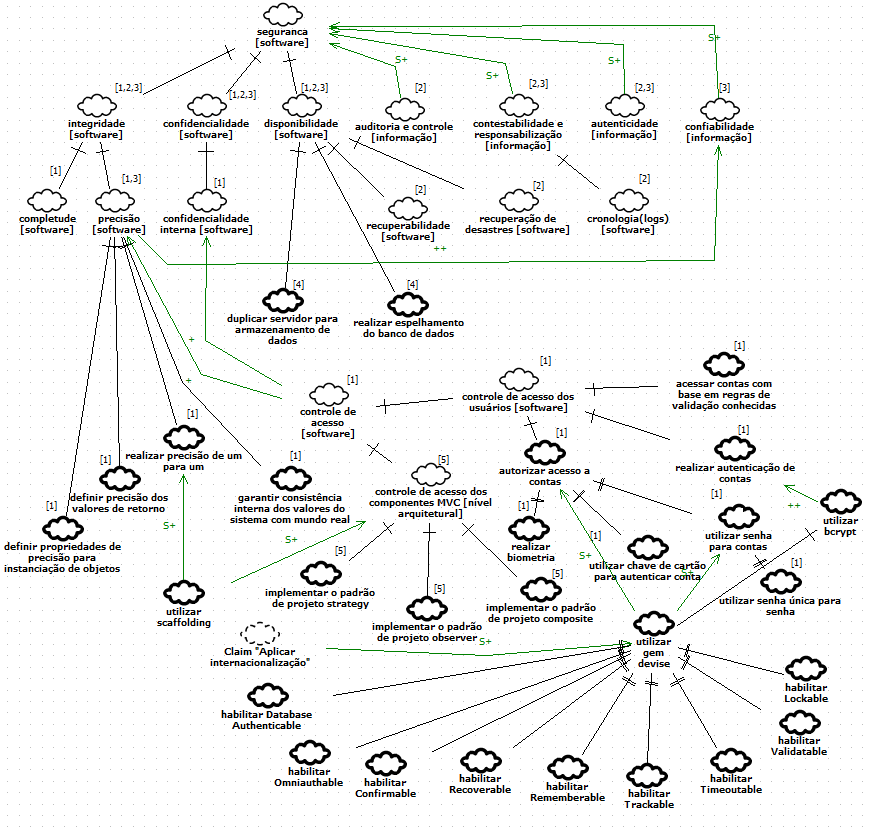
\includegraphics[keepaspectratio=true,scale=0.7]{figuras/catalogoFull.PNG}
	\caption{Versão extendida do catálogo focada em projetos \textit{rails}}
	\label{catalogoFull}
\end{figure}

\pagebreak

No entanto durante a validação do catálogo foi utilizado projetos reais e abstrações de possíveis usuários e cenários tornando o catálogo mais abrangente caso a tecnologia utilizada seja o \textit{rails}, como um exemplo de evolução do catálogo e as evidências comprovadas da relação entre as operacionalizações e as camadas do padrão arquitetural MVC é possível unificar com fins de demonstração o Catálogo de Segurança com um diagrama de componentes do padrão MVC, onde as operacionalizações estão dentro do componente ao qual possui relacionamento, como pode ser visualizado na Figura \ref{catalogoMapeado}. 


\begin{comment}
	A Tabela \ref{resultadosObtidos} apresenta de acordo com os objetivos específicos do trabalho, usando "atendido", "parcialmente atendido" e "não atendido", os principais resultados obtidos até o momento, com a realização do TCC1.	
\end{comment}

\begin{figure}[h!]
	\centering
	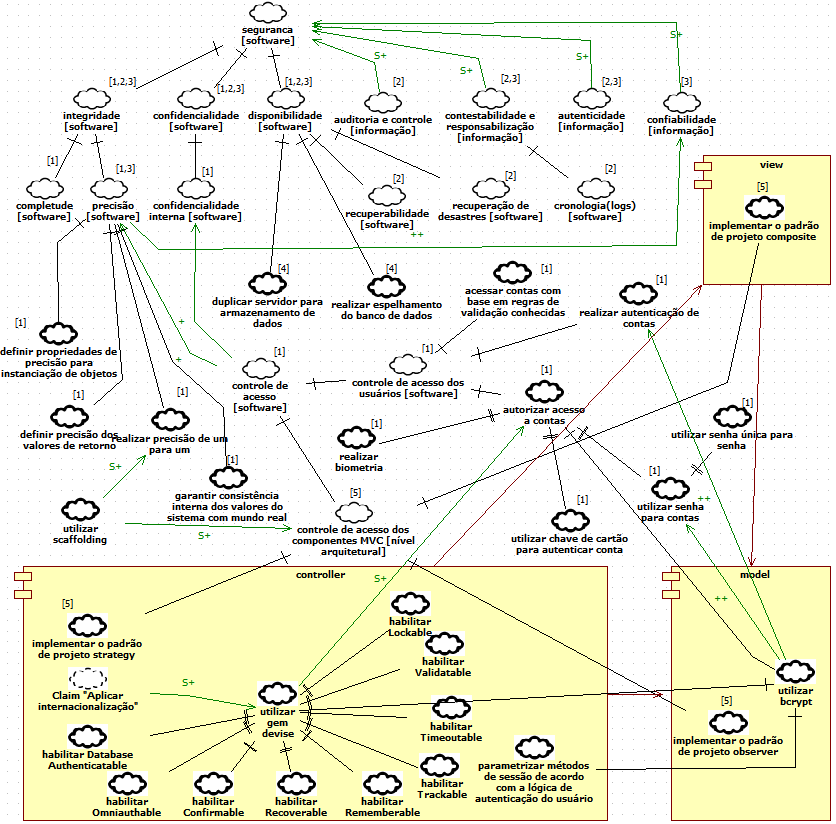
\includegraphics[keepaspectratio=true,scale=0.7]{figuras/catalogoMapeado.PNG}
	\caption{Mapeamento das metas flexíveis e operacionalizações com as camadas do MVC.}
	\label{catalogoMapeado}
\end{figure}


\begin{comment}
	\begin{table}[h!]
	\centering
	\caption{Resultados obtidos de acordo com os objetivos específicos.}
	\label{resultadosObtidos}
	\tiny
	\begin{tabular}{@{}p{6cm}p{3cm}p{6cm}@{}}
	\toprule
	\textbf{Objetivo} & \textbf{Nível de satisfação} & \textbf{Motivo} \\ \midrule
	Investigar na literatura formas de lidar com o RNF Segurança  em aplicações Web desenvolvidas utilizando o MVC. & Parcialmente atendido & Parcialmente atendido, pois existem fontes não confiáveis que comprovam o impacto do RNF Segurança com aplicações web desenvolvidas utilizando o MVC, um exemplo claro de fonte não confiável são os fóruns de dúvidas. Considera-se que ao desenvolver a aplicação fica mais evidente e possível comprovar as formas de lidar com o RNF segurança no Padrão arquitetural MVC. \\
	\rowcolor[HTML]{C0C0C0} 
	Investigar na literatura os RNF associados a segurança e identificar o impacto e as interdepêndencias entre eles. & Parcialmente atendido & Parcialmente atendido, pois a subjetividade dos RNFs para Segurança dificulta o tratamento, além de dificultar a identificação do impacto entre eles. \\
	Elaborar SIG & Atendido & Atendido, pois tem-se a primeira versão do catálogo elaborado com sucesso. \\
	\rowcolor[HTML]{C0C0C0} 
	Realizar correspondência entre o catálogo e as camadas do padrão arquitetural MVC & Atendido & Atendido, pois essa correspondência foi analisada de acordo com a base teórica já levantada. \\ \bottomrule
	\end{tabular}
	\end{table}
\end{comment}

